\documentclass{article}

\usepackage[left=2cm,right=2cm, top=2cm, bottom = 2cm]{geometry}
\usepackage{amsfonts}
\usepackage{amsmath}
\usepackage{array}

\usepackage{tikz}

\newcommand{\cosec}{\mathrm{cosec}}

\pagestyle{empty}

%\setlength{\tabcolsep}{0.8cm}
\renewcommand{\arraystretch}{1.3}

\makeatletter
\newcommand{\thickhline}{%
    \noalign {\ifnum 0=`}\fi \hrule height 2pt
    \futurelet \reserved@a \@xhline
}
\newcolumntype{!}{@{\hskip\tabcolsep\vrule width 2pt\hskip\tabcolsep}}
\makeatother

\begin{document}

\title{Solving Trig Equations}
\date{}

\maketitle

\Large

{\bf \underline{Objective: To be able to solve equations with trig functions.}}

\vspace{5mm}



{\bf Recap of previous material:}

\vspace{5mm}

\begin{enumerate}
\item $\sin\left(\frac{\pi}{4}\right)=$
\item $\cos\left(\frac{\pi}{6}\right)=$
\item $\tan\left(\frac{\pi}{3}\right)=$
\item Sketch the graph of $y=\sec(x)$.
\item Sketch the graph of $y=\cot(x)$.
\end{enumerate}


\clearpage






{\bf Warm-up:}

\vspace{5mm}

\begin{enumerate}
\item For what values of $x$ does $\sin(x)=0$?
\item For what values of $x$ does $\cos(x)=-1$?
\item Solve $\sin(x)=\frac{\sqrt{3}}{2}$ for $0\leq x<2\pi$.
\item Solve $\cos(x)=\frac{1}{2}$ for $0\leq x<2\pi$.
\item Find $\theta$ between $0$ and $2\pi$ such that $\cos(\theta)=\frac{1}{2}$ and $\sin(\theta)=\frac{\sqrt{3}}{2}$.
\end{enumerate}

\clearpage


{\bf Worked Examples - Solving Trig Equations:}

\vspace{5mm}

Solve $\sec(t)-9=\cos(t)$ for $0\leq t<2\pi$:

\vfill


Solve $\cot(\theta+30^\circ)=\sqrt{3}$ for $0\leq \theta<360^\circ$:

\vfill



\clearpage






\textbf{Practice:}

\vspace{5mm}

\begin{enumerate}
\item Solve $\sin(x)+2=3$ for $0^\circ \leq x < 360^\circ$
\item Solve $2\cos^2(x)-\sqrt{3}\cos(x)=0$ for $0\leq x<2\pi$.
\item Solve $\sin^2(\theta)-\sin(\theta)=2$ for $0\leq x<2\pi$.
\item Solve $\cos^2(t)+\cos(t)=\sin^2(t)$ for $0\leq t<2\pi$.
\item Solve $\cosec(x)+a\sin(x)=b$ in terms of $a$ and $b$, for $0^\circ\leq x<360^\circ$.
\end{enumerate}






\clearpage

\textbf{Application---Orbital Motion:}

\vspace{5mm}


The planet Zorg orbits its star in a circular orbit; its position at time $t$ is given by
\[x(t)=r\cos\left(\frac{2\pi}{T}t\right),\qquad\qquad y(t)=r\sin\left(\frac{2\pi}{T}t\right),\]
where $T$ is the orbital period (the length of one year on the planet), and $r$ is the radius of the orbit. The coordinate axes are set up so that the sun is at the origin.

The planet Yarg orbits the same star with radius $\frac{r}{2}$ and period $\frac{T}{2}$, and out of phase. Its position at time $t$ is given by
\[x(t)=\frac{r}{2}\cos\left(\frac{4\pi}{T}t+\frac{\pi}{2}\right),\qquad\qquad y(t)=\frac{r}{2}\sin\left(\frac{4\pi}{T}t+\frac{\pi}{2}\right).\]


An astronaut plans to fly from Zorg to Yarg, and wants to do so when the distance between the planets is minimum, to save fuel.

\begin{enumerate}
\item Write down an expression for $\Delta x$ (the difference in $x$-coordinates of the two planets), and a similar expression for $\Delta y$, the difference in $y$-coordinates.
\item Hence write down an expression for the distance $d$ between the two planets at time $t$. Simplify this expression.
\item Using the formulae
	\[\cos(A)\cos(B)=\frac{1}{2}(\cos(A+B)+\cos(A-B)),\]
	\[\sin(A)\sin(B)=\frac{1}{2}(\cos(A-B)-\cos(A+B)),\]
	simplify your expression for the distance further.
\item The distance is a minimum (respectively maximum) precisely when the square of the distance is minimum (respectively maximum), and the square of the distance is easier to work with. 		Show that, for $0\leq t<T$ the distance attains its minimum and maximum values when
	\[\sin\left(\frac{2\pi}{T}t+\frac{\pi}{2}\right)=0.\]
	Note: If you haven't yet done differentiating trig functions or maximum/minimum problems, skip this part.
\item Solve the equation in part 4 for $0\leq t<T$.
\item Hence say when the astronaut should make their flight.
\end{enumerate}

% xdiff=r|\cos(2t\pi/T)-(1/2)\cos(4t\pi/T+\pi/2)|, ydiff=r|\sin(2t\pi/T)-(1/2)\sin(4t\pi/T+\pi/2)
% dist=r\sqrt{\cos^2(2t\pi/T)-\cos(2t\pi/T)\cos(4t\pi/T+\pi/2)+(1/4)\cos^2(4t\pi/T+\pi/2)+\sin^2(2t\pi/T)-\sin(2t\pi/T)\sin(4t\pi/T+\pi/2)+(1/4)\sin^2(4t\pi/T+\pi/2)} = r\sqrt{(5/4)-(\cos(4t\pi/T+\pi/2)\cos(2t\pi/T)+\sin(4t\pi/T+\pi/2)\sin(2t\pi/T))}
% dist = r\sqrt{(5/4)-(1/2)(\cos(5t\pi/T+\pi/2)+\cos(3t\pi/T+\pi/2) + \cos(3t\pi/T+\pi/2)-\cos(5t\pi/T+\pi/2))} = r\sqrt{(5/4)-\cos(3t\pi/T+\pi/2)}
% dist^2 =r^2((5/4)-\cos(3t\pi/T+\pi/2)). deriv=(3\pi/T)r^2\sin(3t\pi/T+\pi/2)

\clearpage



\textbf{Solution:}

\vspace{5mm}

\begin{enumerate}
\item \[\Delta x=r\left(\cos\left(\frac{2\pi}{T}t\right)-\frac{1}{2}\cos\left(\frac{4\pi}{T}t+\frac{\pi}{2}\right)\right)\]
	\[\Delta y=r\left(\sin\left(\frac{2\pi}{T}t\right)-\frac{1}{2}\sin\left(\frac{4\pi}{t}t+\frac{\pi}{2}\right)\right)\]
\item For clarity, write $\alpha=\frac{2\pi}{T}t$ and $\beta=\frac{4\pi}{T}t+\frac{\pi}{2}.$
	\begin{align*}
	d&=\sqrt{(\Delta x)^2+(\Delta y)^2}\\
	&= r\sqrt{\cos^2(\alpha)-\cos(\alpha)\cos(\beta)+\frac{1}{4}\cos^2(\beta)+\sin^2(\alpha)-\sin(\alpha)\sin(\beta)+\frac{1}{4}\sin^2(\beta)}\\
	&=r\sqrt{\cos^2(\alpha)+\sin^2(\alpha) + \frac{1}{4}(\cos^2(\beta)+\sin^2(\beta))-\cos(\alpha)\cos(\beta)-\sin(\alpha)\sin(\beta)}\\
	&=r\sqrt{\frac{5}{4}-\cos(\alpha)\cos(\beta)-\sin(\alpha)\sin(\beta)}
	\end{align*}
\item \begin{align*}
	d&=r\sqrt{\frac{5}{4}-\frac{1}{2}(\cos(\alpha+\beta)+\cos(\alpha-\beta))-\frac{1}{2}(\cos(\alpha-\beta)-\cos(\alpha+\beta))}\\
	&=r\sqrt{\frac{5}{4}-\frac{1}{2}(2\cos(\alpha-\beta))}\\
	&= r\sqrt{\frac{5}{4}-\cos\left(\frac{-2\pi}{T}t-\frac{\pi}{2}\right)}\\
	&= r\sqrt{\frac{5}{4}-\cos\left(\frac{2\pi}{T}t+\frac{\pi}{2}\right)}
	\end{align*}
\item \begin{align*}
	r^2&=\frac{5}{4}-\cos\left(\frac{2\pi}{T}t\frac{\pi}{2}\right)\\
	\frac{d\,(r^2)}{d\,t}&=\frac{2\pi}{T}\sin\left(\frac{2\pi}{T}t+\frac{\pi}{2}\right)\\
	\end{align*}
	Maxima and minima occur when the derivative is 0, so when
	\[\frac{2\pi}{T}\sin\left(\frac{2\pi}{T}t+\frac{\pi}{2}\right)=0.\]
	Cancelling the factor of $\frac{2\pi}{T}$ gives the desired result.
\item We need to solve
	\[\sin\left(\frac{2\pi}{T}t+\frac{\pi}{2}\right)=0.\]
	for $0\leq t<T$. Let $z=\frac{2\pi}{T}t+\frac{\pi}{2}$, so we need to solve $\sin(z)=0$ for $\frac{\pi}{2}\leq z<\frac{5\pi}{2}$.
	The solutions to this are $z=\frac{n\pi}{2}$ for $n=1,2,3,4$. Hence the $t$-solutions are:
	\[t=\frac{(n-1)T}{4}\qquad\mbox{ for }\qquad n=1,2,3,4.\]
\item We need to identify which of the above times gives a global minimum. We can do this by evaluating the distance (or the squared distance) at each of those times, and picking the smallest value. (Note: if you know the 2nd derivative test, we could also use that first to reduce the possibilities to check). We have:
	\begin{center}
	\begin{tabular}{c|c|c|c}
	$n$ & $t$ & $z$ & $d$ \\ \thickhline
	1 & 0 & $\frac{\pi}{2}$ & $\frac{\sqrt{5}}{2}r$\\ \hline
	2 & $\frac{T}{4}$ & $\pi$ & $\frac{3}{2}r$\\ \hline
	3 & $\frac{T}{2}$ & $\frac{3\pi}{2}$ & $\frac{\sqrt{5}}{2}r$\\ \hline
	4 & $\frac{3T}{4}$ & $2\pi$ & $\frac{1}{2}r$
	\end{tabular}
	\end{center}
\end{enumerate}

\begin{center}
\begin{tikzpicture}[scale=0.8]
\draw[fill,yellow] (0,0) circle[radius = 0.5];
\draw[gray,->] (-5,0) -- (5,0);
\node[right] at (5,0) {$x$};
\draw[gray,->] (0,-5) -- (0,5);
\node[above] at (0,5) {$y$};

\draw[fill,blue] (4,0) circle[radius=0.1];
\node[above, blue] at (4,0) {Zorg};
\draw[dashed,blue] (0,0) circle[radius=4];

\draw[fill,red] (0,2) circle[radius=0.1];
\node[right,red] at (0,2) {Yarg};
\draw[dashed, red] (0,0) circle[radius=2];

\node[below right] at (4,0) {$r$};
\node[below] at (2,0) {$\frac{r}{2}$};

\draw[<->,dashed, thick] (3.8,0.1) -- (0.2,1.9);
\node[above] at (2,1) {$d$};

\node at (0,-6) {$t=0$};
\end{tikzpicture}
\end{center}



\begin{center}
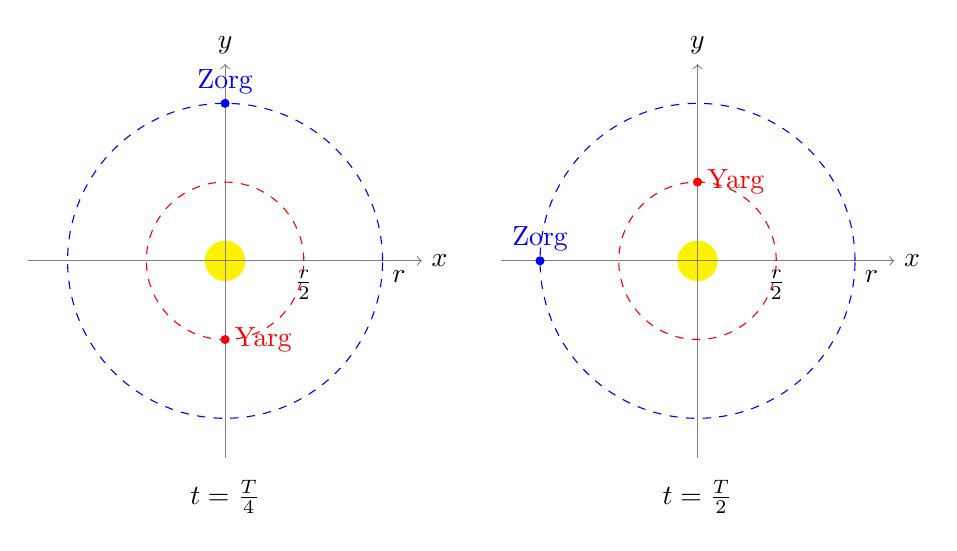
\begin{tikzpicture}[scale = 0.5]
\draw[fill,yellow] (0,0) circle[radius = 0.5];
\draw[gray,->] (-5,0) -- (5,0);
\node[right] at (5,0) {$x$};
\draw[gray,->] (0,-5) -- (0,5);
\node[above] at (0,5) {$y$};

\draw[fill,blue] (0,4) circle[radius=0.1];
\node[above, blue] at (0,4) {Zorg};
\draw[dashed,blue] (0,0) circle[radius=4];

\draw[fill,red] (0,-2) circle[radius=0.1];
\node[right,red] at (0,-2) {Yarg};
\draw[dashed, red] (0,0) circle[radius=2];

\node[below right] at (4,0) {$r$};
\node[below] at (2,0) {$\frac{r}{2}$};

\node at (0,-6) {$t=\frac{T}{4}$};

\draw[fill,yellow] (12,0) circle[radius = 0.5];
\draw[gray,->] (7,0) -- (17,0);
\node[right] at (17,0) {$x$};
\draw[gray,->] (12,-5) -- (12,5);
\node[above] at (12,5) {$y$};

\draw[fill,blue] (8,0) circle[radius=0.1];
\node[above, blue] at (8,0) {Zorg};
\draw[dashed,blue] (12,0) circle[radius=4];

\draw[fill,red] (12,2) circle[radius=0.1];
\node[right,red] at (12,2) {Yarg};
\draw[dashed, red] (12,0) circle[radius=2];

\node[below right] at (16,0) {$r$};
\node[below] at (14,0) {$\frac{r}{2}$};

\node at (12, -6) {$t=\frac{T}{2}$};
\end{tikzpicture}
\end{center}


\begin{center}
\begin{tikzpicture}[scale=0.8]
\draw[fill,yellow] (0,0) circle[radius = 0.5];
\draw[gray,->] (-5,0) -- (5,0);
\node[right] at (5,0) {$x$};
\draw[gray,->] (0,-5) -- (0,5);
\node[above] at (0,5) {$y$};

\draw[fill,blue] (0,-4) circle[radius=0.1];
\node[above, blue] at (0,-4) {Zorg};
\draw[dashed,blue] (0,0) circle[radius=4];

\draw[fill,red] (0,-2) circle[radius=0.1];
\node[right,red] at (0,-2) {Yarg};
\draw[dashed, red] (0,0) circle[radius=2];

\node[below right] at (4,0) {$r$};
\node[below] at (2,0) {$\frac{r}{2}$};

\node at (0,-6) {$t=\frac{3T}{4}$};
\end{tikzpicture}
\end{center}



\clearpage












\end{document}